%%%%%%%%%%%%%%%%%%%%%%%%%%%%%%%%%%%%%%%%%%%%%%%%%%%%%%%%%%%%%%%%%%%%%%%%%%%%%%%%%%%%%%%%%%%%%%%%%%%
% Appendix -> Supplementary Tables and Figures
% Author: Mingbo Cheng
%%%%%%%%%%%%%%%%%%%%%%%%%%%%%%%%%%%%%%%%%%%%%%%%%%%%%%%%%%%%%%%%%%%%%%%%%%%%%%%%%%%%%%%%%%%%%%%%%%%
\chapter{Appendix}
\label{chapter:appendix}

\setstretch{1}

\graphicspath{{appendix/figs}}



\begin{table*}[ht]
\centering
\caption[Time consumption of MOJITOO]{Benchmarking experiments on SKIN-SHARE data set (time elapsed in minutes). Of note LIGER could only be executed with up to 28,147 cells. We also include  two versions of MOFA with the full input matrices (MOFA full) or with reduced input matrices (MOFA).}
\begin{tabular}{r|rrrrrrrrr}
  \hline
 cells & DIABLO & LIGER & MOFA-Full & MOFA & MOJITOO & scAI & schema & Symph-Int & WNN \\ 
  \hline
3000 & 2.00 & 0.65 & 1.65 & 0.46 & 0.42 & 5.69 & 2.12 & 0.46 & 0.51 \\ 
  6000 & 6.91 & 1.06 & 3.10 & 0.88 & 0.63 & 15.29 & 4.10 & 0.78 & 0.82 \\ 
  9000 & 13.33 & 1.63 & 4.58 & 1.14 & 0.88 & 33.37 & 4.84 & 1.10 & 1.17 \\ 
  12000 & 21.18 & 2.19 & 7.24 & 1.31 & 1.13 & 62.68 & 5.70 & 1.30 & 1.56 \\ 
  15000 & 28.52 & 2.59 & 11.20 & 1.60 & 1.37 & 121.74 & 6.98 & 1.59 & 1.92 \\ 
  18000 & 40.85 & 3.02 & 18.53 & 2.26 & 1.83 & 171.82 & 8.02 & 2.09 & 2.50 \\ 
  21000 & 53.88 & 3.61 & 34.51 & 2.58 & 2.08 & 249.61 & 9.08 & 2.43 & 2.90 \\ 
  24000 & 69.14 & 4.23 & 43.96 & 2.85 & 2.30 & 350.98 & 10.56 & 2.64 & 3.26 \\ 
  27000 & 89.49 & 4.58 & 52.47 & 3.19 & 2.56 & 485.13 & 11.79 & 2.95 & 3.68 \\ 
  30000 & 103.26 & - & 67.53 & 3.21 & 2.48 & 637.52 & 13.09 & 3.01 & 3.74 \\ 
   \hline
\end{tabular}
\label{tab:time}
\end{table*}


\begin{table*}[ht]
\centering
\caption[Peak Memory of MOJITOO]{Peak memory consumption in gigabytes. Of note LIGER could only be executed with up to 28,147 cells. We also include  two versions of MOFA with the full input matrices (MOFA full) or with reduced input matrices (MOFA)}
\begin{tabular}{r|rrrrrrrrr}
  \hline
 cells & DIABLO & LIGER & MOFA-Full & MOFA & MOJITOO & scAI & Schema & Symph-Int & WNN \\ 
  \hline
3000 & 9.61 & 10.88 & 1.66 & 3.20 & 1.61 & 6.27 & 10.66 & 3.19 & 1.61 \\ 
  6000 & 10.87 & 9.99 & 2.37 & 4.76 & 2.11 & 10.65 & 11.41 & 4.74 & 2.11 \\ 
  9000 & 15.25 & 9.09 & 2.51 & 6.37 & 2.46 & 10.32 & 11.66 & 6.34 & 2.46 \\ 
  12000 & 20.34 & 12.90 & 3.90 & 7.95 & 3.28 & 14.26 & 11.68 & 7.91 & 2.89 \\ 
  15000 & 20.38 & 12.04 & 4.42 & 9.56 & 3.43 & 20.22 & 12.07 & 9.51 & 3.88 \\ 
  18000 & 35.06 & 16.80 & 6.58 & 9.09 & 4.31 & 26.36 & 12.39 & 9.09 & 4.09 \\ 
  21000 & 42.29 & 15.92 & 9.17 & 9.28 & 5.01 & 34.14 & 13.11 & 9.28 & 5.58 \\ 
  24000 & 50.61 & 21.85 & 12.49 & 8.86 & 4.85 & 43.27 & 13.29 & 8.86 & 5.84 \\ 
  27000 & 57.22 & 20.93 & 17.94 & 13.05 & 5.94 & 58.91 & 13.74 & 13.05 & 5.93 \\
  30000 & 78.30 & - & 22.47 & 13.09 & 6.34 & 75.92 & 14.28 & 13.09 & 6.79 \\ 
   \hline
\end{tabular}
\label{tab:memory}
\end{table*}


\begin{figure}[!ht]
	\centering
	\includegraphics[width=0.95\textwidth]{MOFA/fig}
	\vspace{0.1cm}
	\caption[MOFA dimensional reduction comparison.]{MOFA dimensional reduction comparison.}
	\label{fig:MOFA}
\end{figure}


\begin{figure}[!ht]
	\centering
	\includegraphics[width=0.95\textwidth]{Input_Dimensions/fig}
	\vspace{0.1cm}
	\caption[Input dimensions affection]{Input dimension.}
	\label{fig:Input_Dimensions}
\end{figure}






